\chapter{Task Resolution}
This chapter will describe all the tasks handled in this sprint in varying degrees of detail depending on the significance and uniqueness of the solution.
\section{Update Dependencies}
In the current state of the Giraf project the individual sub--project, which are applications or libraries for Android, use a series of common libraries made for the Giraf project.
The dependencies for each application and library are not all updated to use the newest versions of each other, this might cause bugs that are already fixed in a later version.
Consequently since the dependencies are not updates, new bugs may be caused as the newer versions have not been implemented with each other.
Fixing these bugs is a part of the task to update dependencies and must be fixed when doing so.
For this reason the first order of business should be updating and configure the dependencies, such that this year's Giraf project will start with the fewest issues regarding the dependencies.
Subsequently the Product Owner has given these tasks the priority \phigh.
We have estimated these tasks to take 8 EP each for Sequence and Sequence-Viewer, and 16 EP for Picto Search.
We have taken three tasks which relate to upgrading the dependencies of the applications: Sequence and the two libraries Sequence-Viewer and Picto Search.
We took these tasks as they involved common sub--tasks of versions to be upgraded, they are:
\begin{dankscription}{\ttfamily}{meta-database}
    \item[localDB] from version 5.1.2 to 5.1.5
    \item[meta-database] from version 3.2.0 to 3.2.3
    \item[oasisLib] from version 7.2.0 to 9.0.2
\end{dankscription}
\texttt{localDB} is a library which is used to store information in a local database, most of the stored data is received from the remote server when the Giraf Launcher is opened for the first time.
\texttt{localDB}'s purpose is to reduce the inconvenience of having either a slow or no internet connection, however it also introduces some problems in regards to keeping the remote and the local database in sync.
\texttt{meta-database} is used to create the \texttt{localDB}, the changes therein do not affect any of the applications we are tasked with upgrading.
\texttt{localDB} and \texttt{meta-database} have only had their patch-number updated, this indicates a bugfix or small internal corrections as well as backwards compatibility, as such they should not introduce any issues when upgrading.

\texttt{oasisLib} is the library that handles connection from the tablet to the remote database.
In the upgrade from 7.2.0 to 9.0.2 some of the methods used in the applications and libraries were deprecated, and subsequently removed.
One such method is the one which is responsible for loading pictograms, loading pictograms happens to be done through several methods depending on what instance the pictogram is required in.
All uses of these methods have to be replaced with the new method of loading pictograms.
This now uses a helper, \texttt{pictogramHelper}, which has replaced the methods used directly on the model.

\begin{description}
    \item[Sequence--Viewer] \hfill \\
    The Sequence--Viewer used the model directly to get an image, since this method was deprecated when updating \texttt{oasisLib}, it has to be changed.
    This method was used to replace a pictogram in a view after selecting an option from a multiple choice.
    To resolve this issue the line:
\begin{lstlisting}[frame=l]
pictogram.setImage(helper.pictogramHelper.getById(id).getImage());
\end{lstlisting}
was changed to:
\begin{lstlisting}[frame=l]
if(helper.pictogramHelper.getById(id).getName() == null) {
    pictogram.setName("pictogram_name");
} else {
    pictogram.setName(helper.pictogramHelper.getById(id).getName());
}
helper.pictogramHelper.setImage(pictogram,
    helper.pictogramHelper.getImage(
        helper.pictogramHelper.getById(id)));
\end{lstlisting}

    Additionally a null--check have been added to assure that a name, locally, is never set to \texttt{null}, as this can cause issues in other methods which assumes that every pictogram has a name.
    After resolving these issues the application is successfully running as prior to the update.

    \item[Sequence] \hfill \\
    After upgrading sequence to use the newest versions of the libraries mentioned above Sequence was unable to build.
    This was caused by the use of a deprecated method.
    The issue was fixed by changing a single line to use the correct replacement for the deprecated method.
    The code prior to the fix was:
\begin{lstlisting}[frame=l]
pictogram.setImageBitmap(
    helper.pictogramHelper.getById(id).getImage());
\end{lstlisting}
    and the fixed code is:
\begin{lstlisting}[frame=l]
pictogram.setImageBitmap(
    helper.pictogramHelper.getImage(
        helper.pictogramHelper.getById(id)));
\end{lstlisting}

    The line in question is responsible for loading the pictograms from the database into the application.
    Previously the model had been used directly, however in \texttt{oasisLib} 9.0.2 this is no longer supported.
    The method call \texttt{.getById(id)} returns a pictogram object and on that object the \texttt{.getImage()} method is called.
    The \texttt{.getImage()} method has been removed from the pictogram model class in \texttt{oasisLib} 9.0.2, which is why the helper should be used instead.
    After this replacement was made we informally verified that the application worked identically to the previous version with the old dependencies.

    \item[Picto Search] \hfill \\
    After upgrading Picto Search to use the newest dependencies, no issues were found which was not already present in the old version and therefore already on the task list for the multi--project.
    Therefore no changes were made to the application itself during the upgrade.
\end{description}

 With the completion of these tasks, it is now possible to start working on the tasks using these three applications.
 However, we overestimated how much time we would spend on these tasks, we spent a total of 15 EP but had allocated 32 EP for it.
 This task also gave us a deeper understanding of how the Giraf project is structured and how Android applications are structured and written internally.

\subsection{Wiki Migration}
We have the area of responsibility ``Documentation and Wiki'', part of this is ensuring that the information in the Redmine wiki made by the previous GIRAF students is kept since we will depreciate Redmine in favor of Phabricator.
On the Redmine wiki there is a lot of useful information, some of it might be outdated, but most is still useful and should be kept. 

We have taken the task of starting the new wiki on Phabricator, and migrate the useful information from the Redmine wiki to it.
Part of this is to create a structure which the other members of the GIRAF project can use.
It should be noted that the wiki is only used for internal matters inside the GIRAF project.  

It is important that the front page of the wiki is easy to navigate, as this serves as the entry point and from which where all content should be found. 
The contents of the front-page is:

\begin{enumerate}[topsep=0pt,itemsep=-1ex,partopsep=1ex,parsep=1ex]
    \item Actionable Commitments
    \item Guides
    \item GIRAF Project Goals
    \item Useful Links
    \item Sprint Dates
    \item Backlog
    \item Groups and Slack Channels
    \item Wordlist
\end{enumerate}

Most of the content on the wiki are guides which helps the developers with various tasks. 
These should be easy to navigate and have titles which clearly encompass their purpose and content. 
We separate the guides made during this years GIRAF project, which are updated, from the ones made previously. 
Additionally we clearly indicate that the ones constructed previously are not up-to date with the following warning on the top of the page: ``IMPORTANT: This wiki entry has not been updated in 2016''. 

All members of the GIRAF project have access to add to and edit the wiki. 
It is the primary way to share information such as guides and overviews. 
However if this remains unmoderated then the contents of the wiki will most likely become unstructured. 
Therefore in addition the initial migration, we have setup e-mail alerts in Phabricator such that we get a notification every time someone changes the wiki.
Then we will review their additions to ensure that they are located correctly and linked to from the relevant pages etc. 
This will be an ongoing task as part of our area of responsibility.
\subsection{General --- Use Consistent File Encoding}
Throughout GIRAF different file encodings occur, and while this does not impose any problems at the moment, future use of some specific non standard ASCII\footnote{American Standard Code for Information Interchange} text, e.g. Hebraic, can cause build errors and bugs.
The recommended practice by Google is to use UTF-8 encoding on all files to avoid know issues related to other file encodings \footnote{\url{http://tools.android.com/knownissues/encoding}}.

As the files of GIRAF are mostly created on Windows computers, and using older versions of Android Studio, the predominant file encoding across the multi project is Windows-1252 --- an extended version of standard ASCII encoding, including the entire Latin alphabet.
However as GIRAF only uses plain ASCII characters this does not inflict errors, and a full conversion of every file in GIRAF is too severe and intrusive, given the agile nature of the workflow used in the multi project.
This is because rectifying the file encodings, could cause issues such as merge conflicts or unexpected errors.
We therefore propose that changing file encodings to UTF-8 is done as a refactoring step, i.e. when a developer works on a file, he or she checks the encoding and changes it if necessary.
To avoid different practices and inform everybody that they should enforce this change, we write a Wiki entrance describing the process and importance of converting files to UTF-8.

\section{Responsive Search}\label{RSearch}
\userstory{As a User I would like the Picto Search application to feel more responsive when I search for pictograms, such that I don't feel like nothing happens.}

The task is prioritised as \phigh,is estimated at 8 EP, and was created because the customers expressed concern for the reactiveness of the PictoSearch application --- it sometimes felt slow and customers said it felt like nothing was happening.
The PictoSearch application is used whenever the user needs to find a certain pictogram for other applications such as the week schedule or the sequence application.
It is a problem that the users feel like the application is slow and that it does not react quickly to what the user is doing, especially in an application used often by other applications of GIRAF.
It is important that responses from a mobile application are given within a few seconds, as mentioned in~\cite{Roto:2005:NNF:1062745.1062747}, if an application spends more than 4 seconds to load or respond then other feedback than visual should be used.
Therefore the amount of time spent waiting for the application should be reduced, such that there is no need for using other methods of feedback when the search finally returns.
According to Constantine and Lockwood in their book \enquote{Software for Use: A Practical Guide to the Models and Methods of Usage-Centered Design} \cite{DESIGNBOOK}, a design principle regarding feedback is as follows:

\begin{displayquote}
\textit{Keep users informed of actions or interpretations, changes of state or condition and errors or exceptions that are relevant and of interest to the user through clear, concise, and unambiguous language familiar to users\cite[p.~57]{DESIGNBOOK}.}
\end{displayquote}

Therefore it is decided that the Picto Search application should give visual feedback whenever an action occurs.
The application should respond to the users action more often than what it does now to increase how responsive the application feels to the user.

The current version of the PictoSearch application searches whenever the user taps the search button on either the on-screen keyboard or in the GUI of the application.
The search button is located in the middle of the screen, to the left of the search field as can be seen on \myref{fig:screenshot_startup}.

\begin{figure}[h]
    \centering
    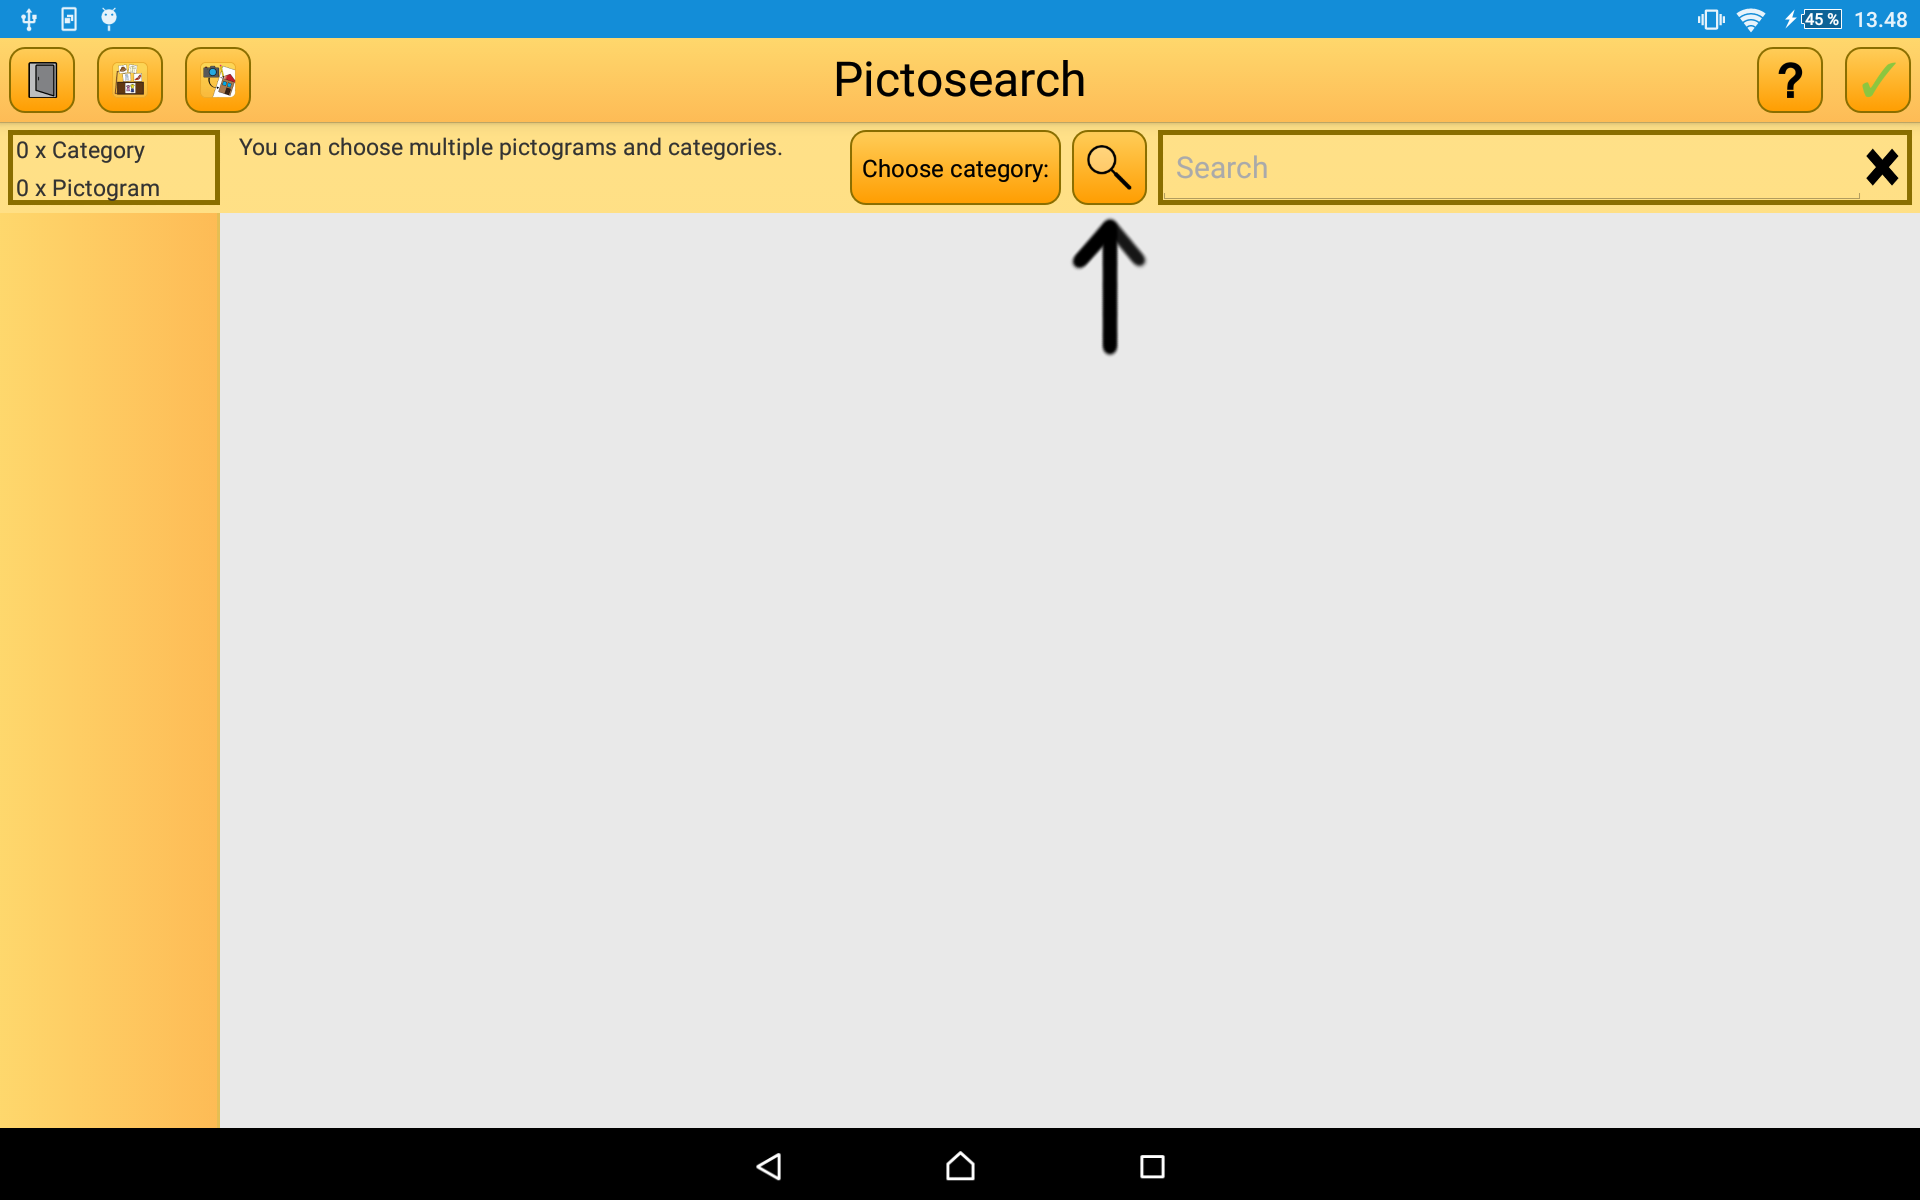
\includegraphics[width=0.8\textwidth]{figures/img/screenshots/old_startup.png}
    \caption{Screenshot of the initial view presented to the user when launching PictoSearch, with the search button highlighted.}\label{fig:screenshot_startup}
\end{figure}
\noindent
The screenshot also shows the view of the application as it is opened, completely empty with no information.

\begin{figure}[h]
    \centering
    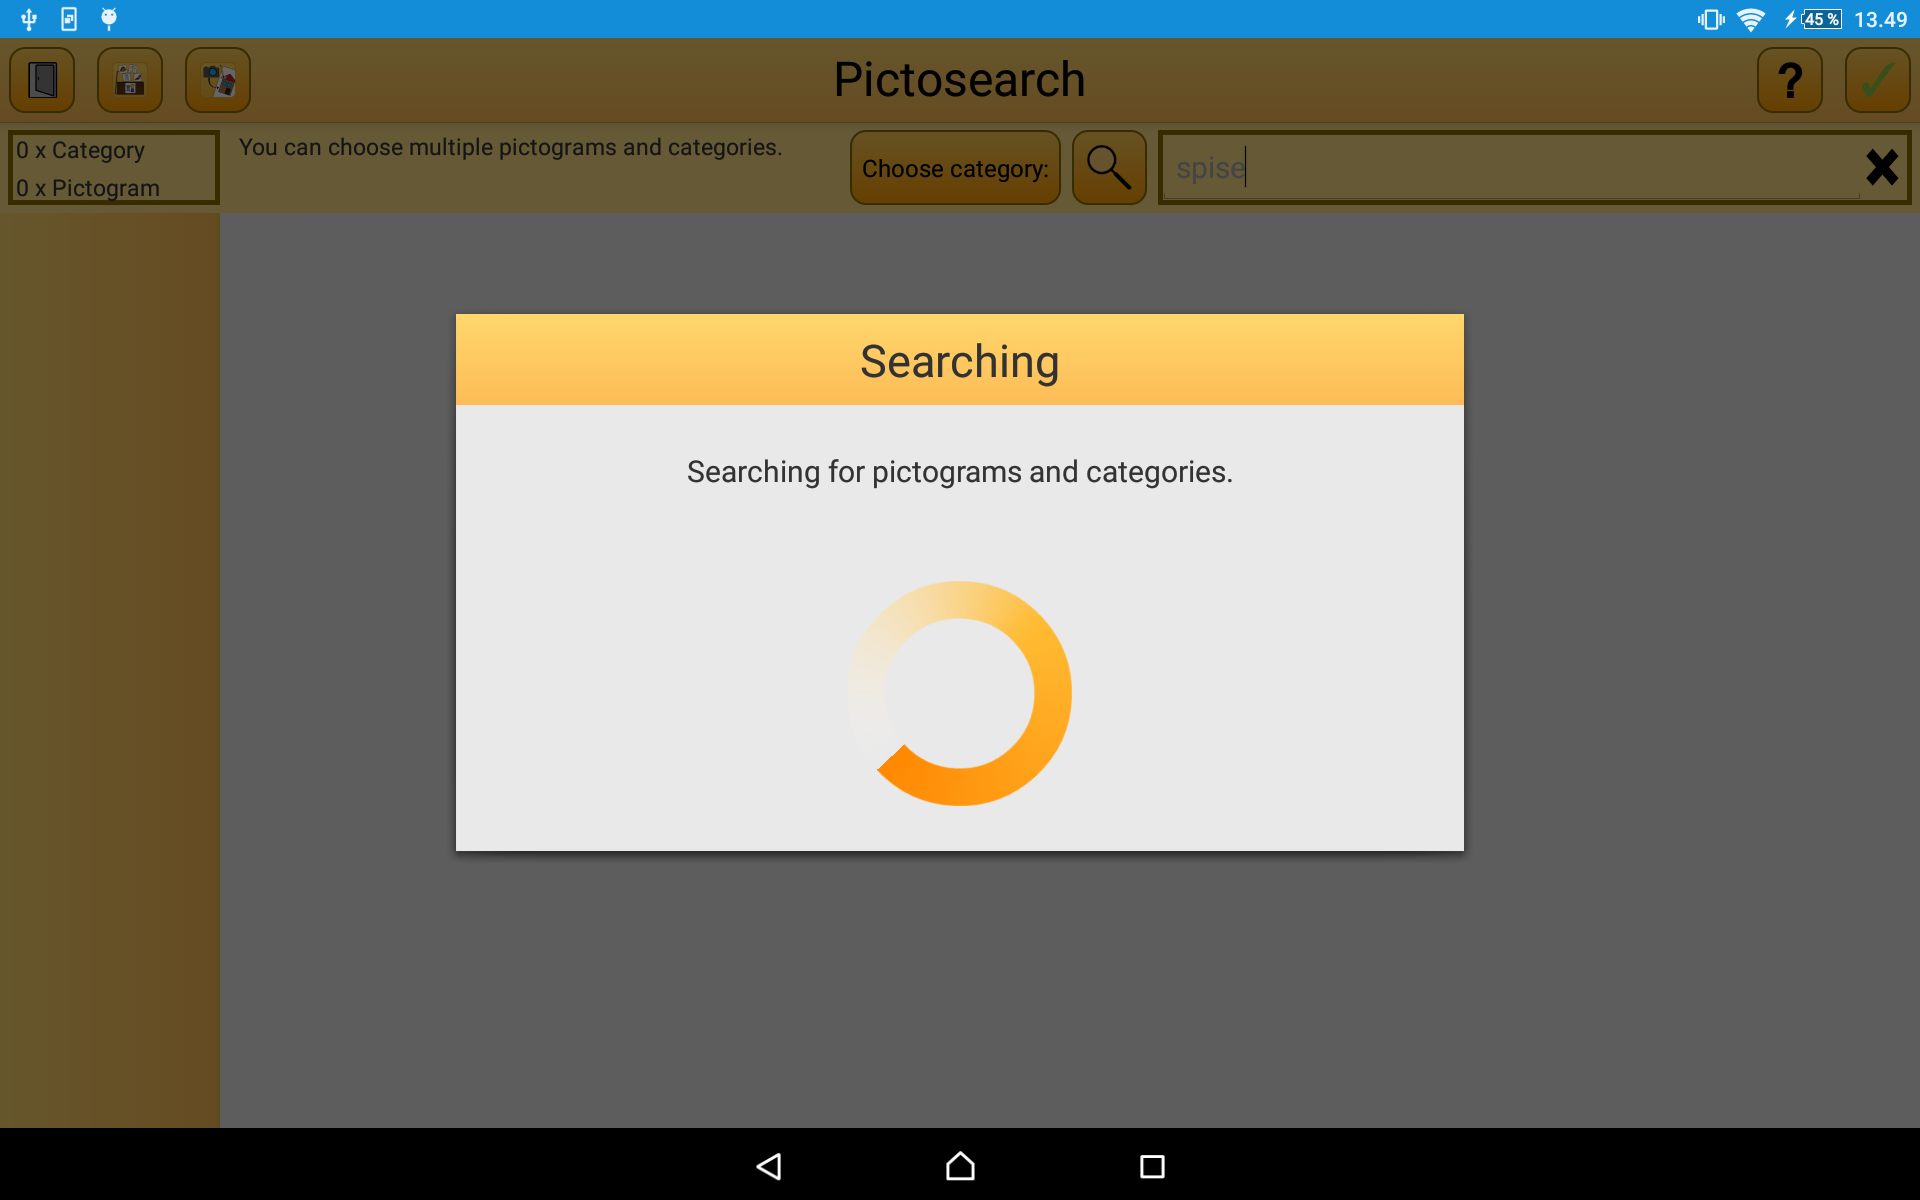
\includegraphics[width=0.8\textwidth]{figures/img/screenshots/old_dialog.png}
    \caption{Screenshot of the search spinner shown while searching in PictoSearch.}\label{fig:screenshot_searchspinner}
\end{figure}

In the new version, a search is made whenever the text in the searchfield is changed.
Instead of the big slow search spinner, which blackened out and locked the screen, shown on \myref{fig:screenshot_searchspinner}, a new smaller text message is instead displayed which tells the user that the application is searching and what is is searching for. 
The current version would also remove the on-screen keyboard when it would search, this only happens in the new version whenever the search button is pressed or the user taps somewhere else, i.e. not on the keyboard.
The application can take input while searching because it is implemented as an async task, i.e. in its own thread.
Because of this any new search is queued behind the current search query, and as such the results of the latest search will be waiting for the results of the previous searches.
This is fixed by a simple change of calling \texttt{AsyncTask.cancel()}, which is a thread.cancellation method, that stops the execution of the ongoing thread and makes it possible to start a new call immediately, with the updated search string, and therefore eliminating the queue.
Because of this anytime a keystroke is made on the keyboard something will happen on the display other than simply filling out the search-field.
When the user types a letter in the textfield, the application will search for the text currently in the text field and display the text as seen on \myref{fig:screenshot_newsearch} explaining what is being searched for. 
This fulfills the principle of giving feedback to the user when an action occurs, such that the user knows what is happening behind the scenes.
When the search returns the pictograms will be shown instead of the text message, with the keyboard still visible.

\begin{figure}[h]
    \centering
    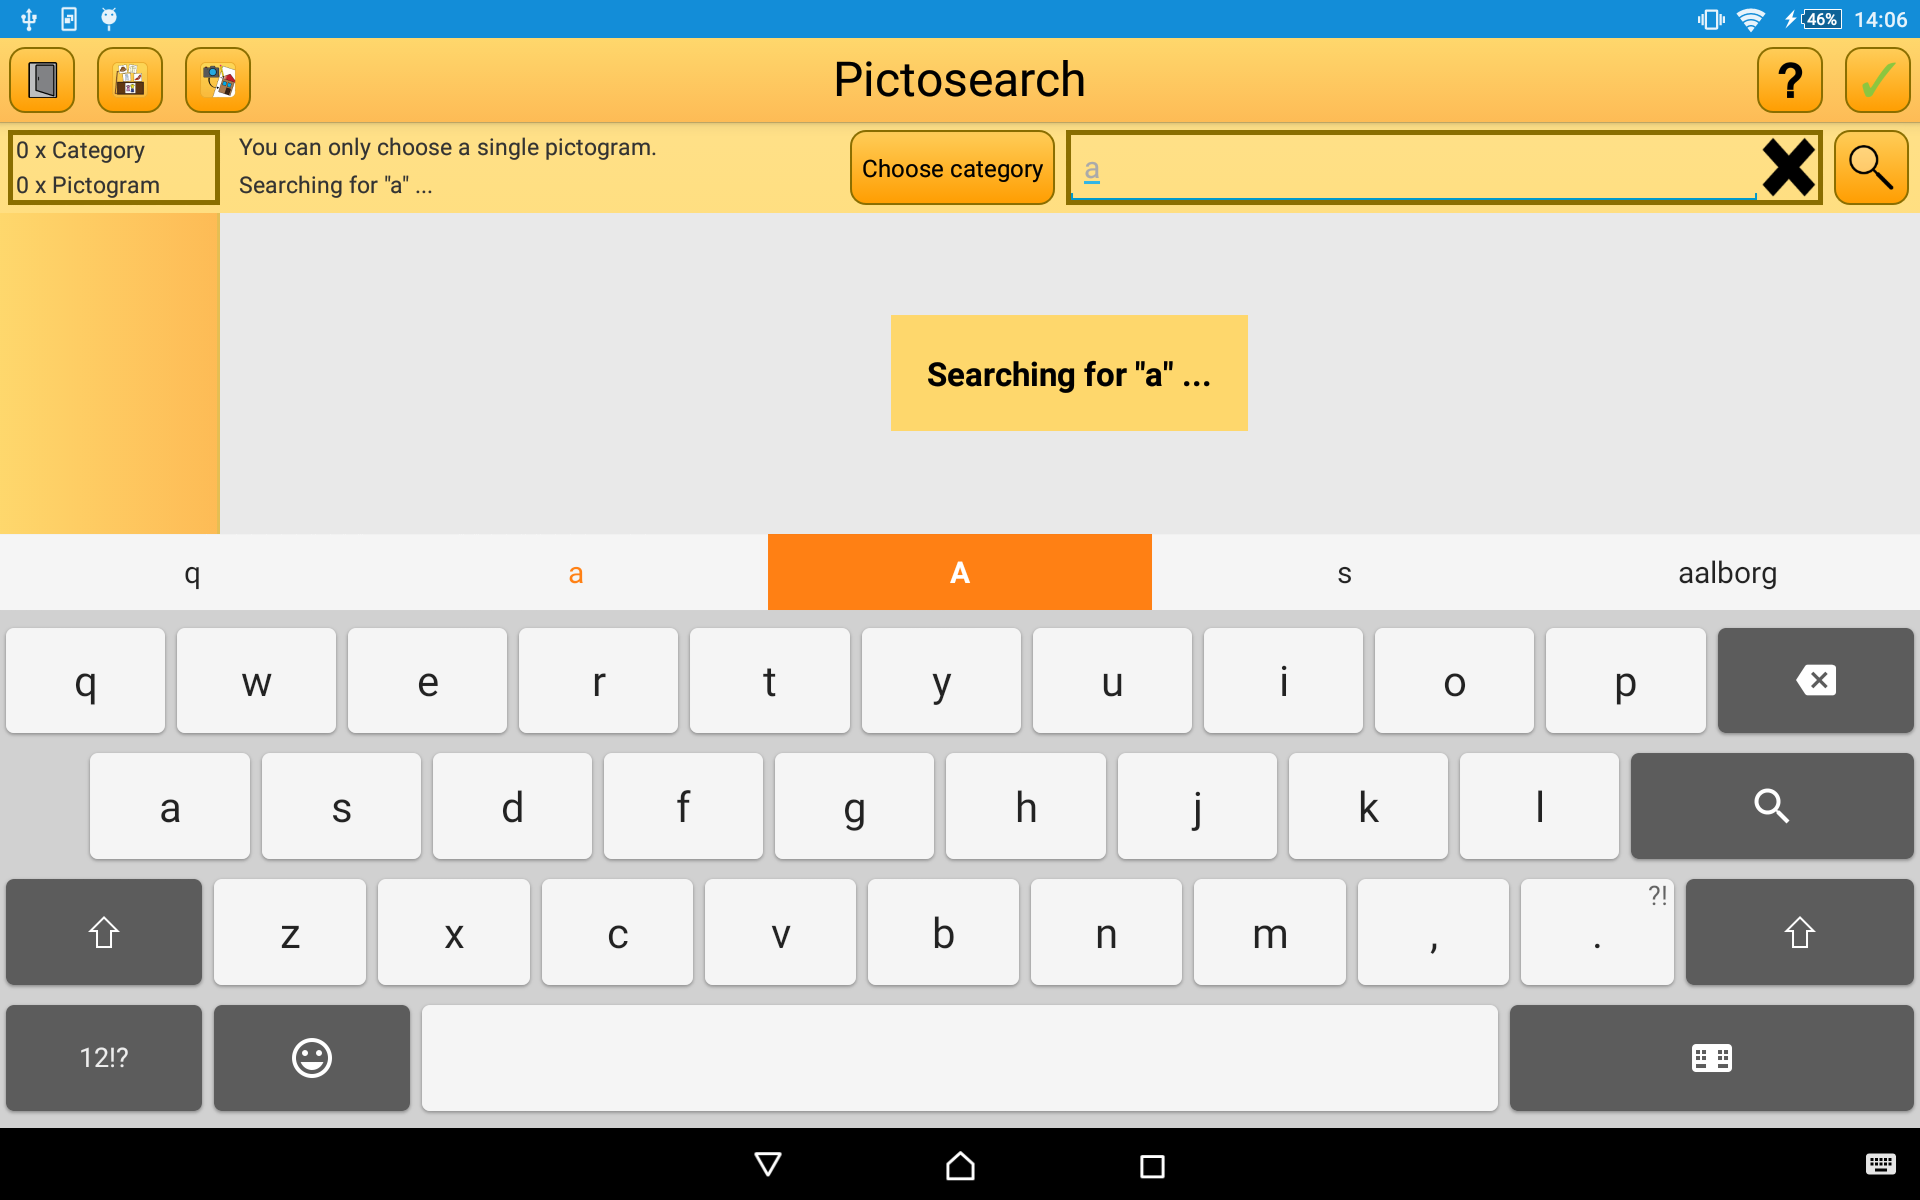
\includegraphics[width=0.8\textwidth]{figures/img/screenshots/new_dialog.png}
    \caption{Screenshot of the new search information, while searching.}\label{fig:screenshot_newsearch}
\end{figure}

This means that there is near instantaneous feedback for the user, which might give the feeling that the application is reacting to whatever the user is doing, and it might no longer feel to users like nothing is happening.
Previously the user would be waiting forever if he thought a search would be performed, when text was entered into the search--field, such as Google does. 
The new approach hereby provides search feedback significantly closer to the aforementioned 4 second limit.
Actually, the query which results in the largest amount of pictograms is a search for the character \enquote{s}, it returns 1932 pictograms and takes approximately 4 seconds on the relatively slow Lenovo tablet provided by the University --- as this is the worst case regarding search time, the average use case will always be faster than 4 seconds. 

The search button can still be used, and will bring up the old search spinner as usually, this is done so that \enquote{refreshing} a search result will provide feedback. 
Moreover the button has been moved from the middle of the display to the right side of the display as can be seen on \myref{fig:screenshot_newstartup}. 
This is a better fit as it resembles other common search engines such as Google Search, and it is also the recommended way to display a search-field according to the Niels Norman Group\footnote{https://www.nngroup.com/articles/magnifying-glass-icon/}.
Furthermore according to the principles of Constantine and Lockwood, structuring the interface is important such that it is for example recognisable: 

\begin{displayquote}
\textit{Organize the user interface purposefully, in meaningful and useful ways based on clear, consistent models that are apparent and recognizable to users, putting related things together and separating unrelated things, differentiating dissimilar things and making similar things resemble one
another.\cite[p.~51]{DESIGNBOOK}.}
\end{displayquote}
\noindent
Therefore using a familiar position of the button is a better fit than placing it in the middle of the screen as in the current version.

Another thing we noticed was that the clear search field button was visible all the time even though no text was in the search field.
This has been removed and it is now only visible when there is text in the search field i.e. when the actoion is available, as can be seen on \myref{fig:screenshot_newstartup} and it it still there on \myref{fig:screenshot_newsearch}.
This has been done because of another design pricinple by Constantine and Lockwood: 

\begin{displayquote}
\textit{Keep all needed options and materials for a given task visible without distracting the user with extraneous or redundant information \cite[p.~55]{DESIGNBOOK}.}
\end{displayquote}

\begin{figure}[h]
    \centering
    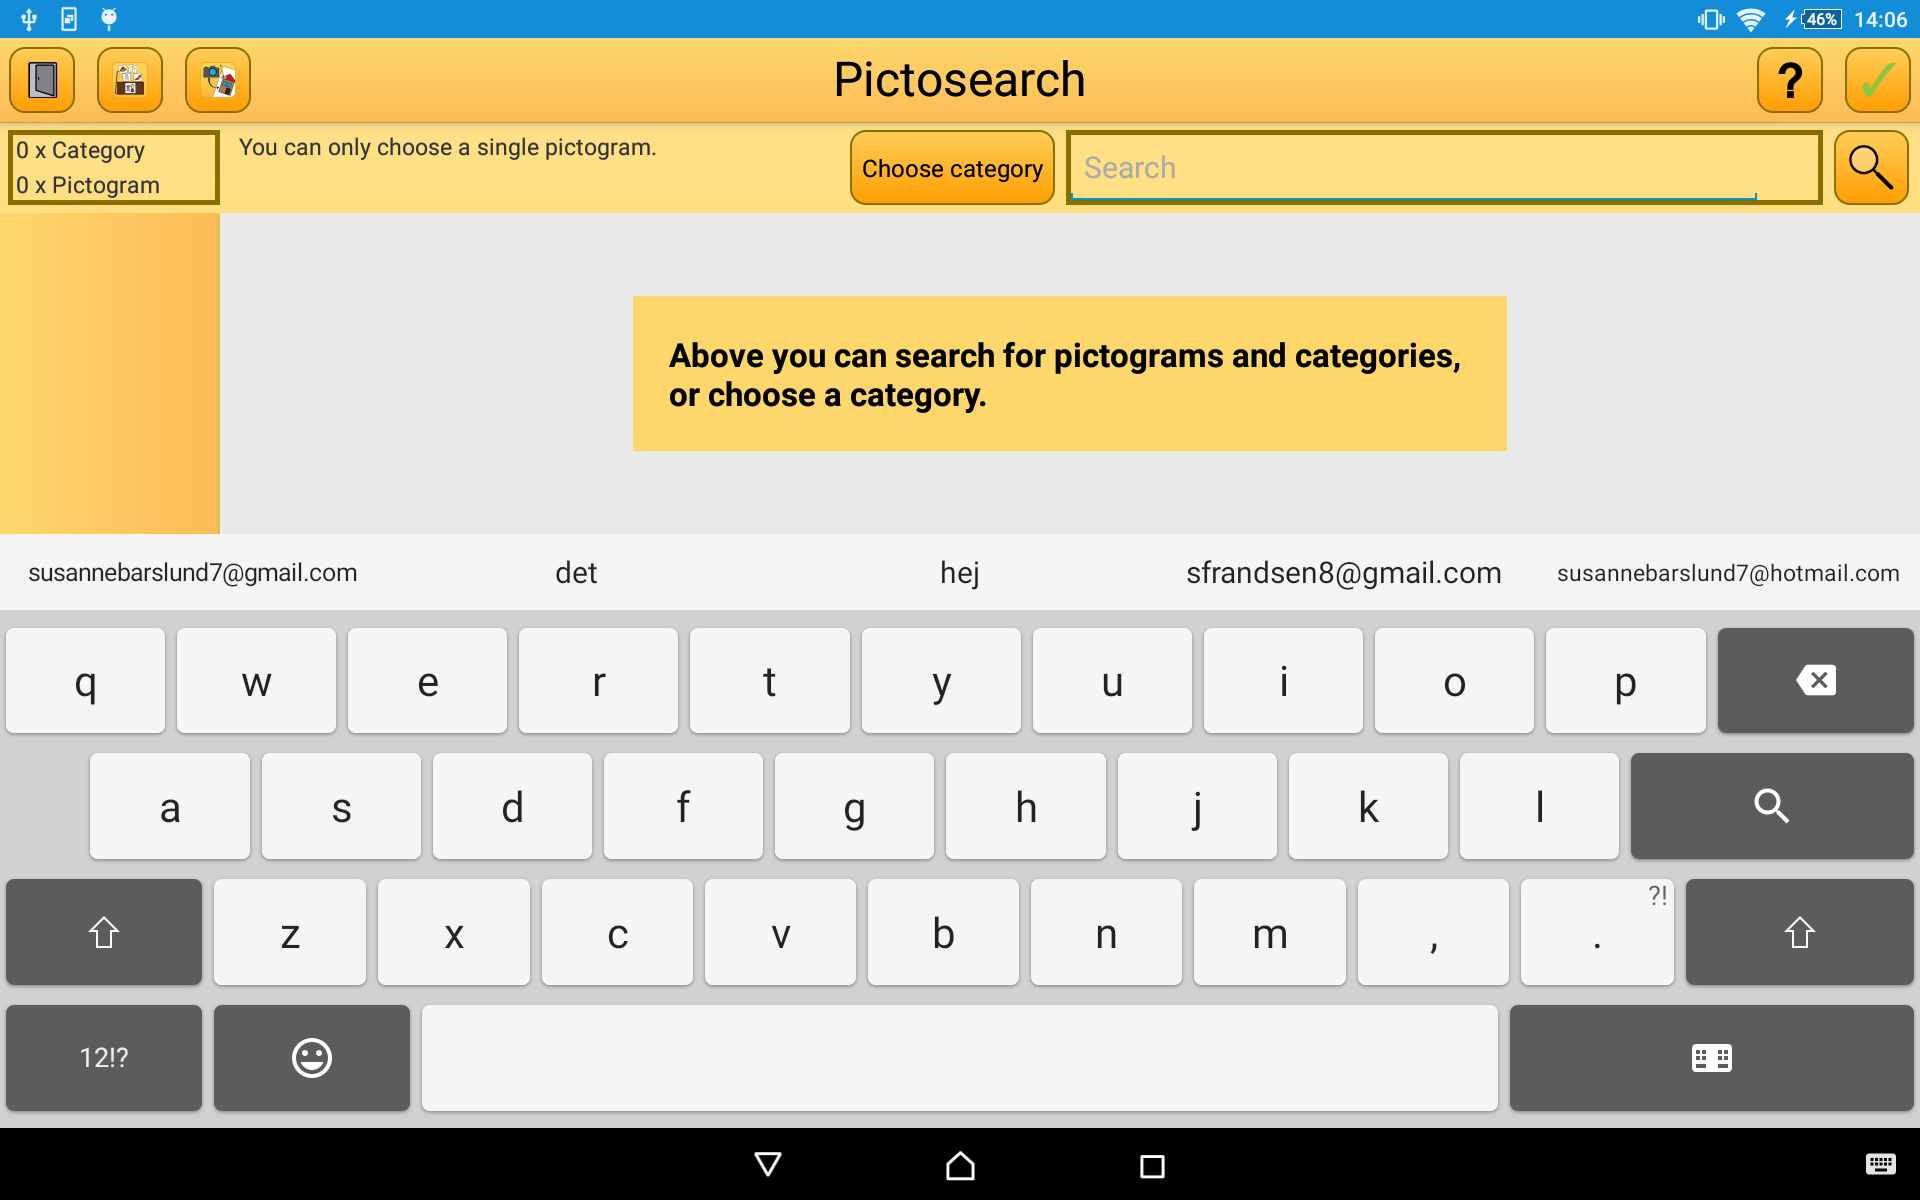
\includegraphics[width=0.8\textwidth]{figures/img/screenshots/new_startup.png}
    \caption{Screenshot of the new initial view in PictoSearch.}\label{fig:screenshot_newstartup}
\end{figure}


\section{It Looks Like There Are No Pictograms, Until You Search For Them}\label{untilSearch}
\section{It Looks Like There Are No Pictograms, Until You Search For Them}\label{untilSearch}
\begin{center}
	\userstory{As a user I would like to have some information when I open Picto Search, such that it does not look like there is nothing there.}
\end{center}

The task is prioritised as \phigh~and has been estimated at 8 EP.  
It should be noted that users of Picto Search always are Guardians.
In the current version, the user is presented with no useful information in the initial view as seen in \myref{fig:screenshot_startup}. 
The view is completely empty, there is no indication that searching is an option apart from the search button, but it does not indicate what you can search for nor how to use the search feature.
This is a problem as the users might feel the application is empty, and may be confused as they do not know how to proceed.
When a user launches Picto Search it is to search for pictograms which are to be used in other applications.
Helping the user by hinting at what to do is deemed a good approach in providing the user with information.
This can be done in two ways, without text and with text:
\begin{description}
    \item [Without text] \hfill\\
    For example when Picto Search is opened the search field could already be in focus and the on-screen keyboard could be shown, effectively reducing the number of actions needed in the search workflow and informs the user that they need to type something.
    \item [With text] \hfill\\
    The other approach is showing text to the user telling them what to do, but this approach alone may not be enough as according to Nielsen \cite{nielsen2003usability} a wall of text is deadly for an interactive experience.
\end{description}

Even though the amount of text in the text solution would be insignificant, it still might not work for all users, so an approach combining both solutions is chosen.
Therefore when Picto Search is opened the software keyboard is forced to appear, along with giving focus to the search field; this enables the user to start searching right away without having to tap anything.
By doing this Picto Search is clearly presented to the user as a search tool similarly to the integrated search function of the iOS mobile operating system, which also shows the keyboard and focusses on the search field upon launch\footnote{\url{https://support.apple.com/en-us/HT201285}}.               
A short description of how Picto Search is operated is also shown in the middle of the screen, hereby providing user with information if they are unsure of how to proceed.
The new view can be seen on \myref{fig:screenshot_newstartup}.
The changes to Picto Search described in this section will be evaluated by the users at the sprint review, along side the previously presented modifications from \myref[name]{RSearch}.
\section{Week Schedule --- Unmark Schedule When Delete is Canceled}
Week Schedule is the only app of GIRAF which this task affects; and the problem occurs in two scenarios:
When a guardian launches Week Schedule they are first prompted to select the citizen for which he wishes to edit schedules.
A view consisting of the concerned citizen's schedules is then presented to the guardian.
In this view the guardian can, among other functions, delete one or more schedules related to the citizen.
This action is performed by tapping the bin in the upper left corner, followed by tapping schedules to mark them for deletion.
When the marking is done the guardian must tap the bin again prompting them with the choice of either completing or canceling the deletion.
In the current version of Week Schedule the cancellation of a delete does not unmark the marked schedules, hereby presenting outdated and confusing feedback to the user.
The same problem is present in the individual schedules when the guardian wants to delete one or more activities from a given schedule, the workflow is the same.
This is formulated as follows:
\begin{center}
\userstory{In Week Schedule as an administrator, I would like week schedules that I marked while in deletion mode to get unmarked if I cancel the delete.}
\end{center}

\subsubsection{Clearing the data}
Most of the prerequisites to solve this issue is already implemented in the current version of Week Schedule for other purposes.
Thus reusing methods which already exist can mostly solve this issue.
In both of the previously described scenarios where wrongful feedback is given, Week Schedule uses two variables respectively called \texttt{markedSchedules} and \texttt{markedActivities} to store the marking.
The \texttt{markedSchedules} is a \texttt{HashSet} of booleans related to each of the schedules available for marking; and clearing the \texttt{HashSet} is done by simply calling \texttt{.clear()} on the \texttt{HashSet}--object.
With the \texttt{markedActivities} variable, clearing the marking proved to be the more difficult scenario.
Since \texttt{markedActivities} is implemented as an \texttt{ArrayList} with each element being a boolean array, the \texttt{.clear()} did not behave in the same way.
In the \texttt{ArrayList} each boolean array represents a day on the schedule, which means that clearing the entire \texttt{ArrayList} will remove all existing boolean arrays; this will then cause out of bounds exceptions later on if the user tries to make a new marking, because the boolean arrays have zero elements.
Hence a custom implementation of a clear method can be used to solve the issue.
This is done by filling the \texttt{ArrayList}, \texttt{markedActivities}, with new boolean arrays of appropriate sizes and with the default boolean value being false.
This ensures that future markings can be made without crashing the application.
These changes will are not enough to present the user with the appropriate feedback just yet as the view must also be updated.
The clearing is handled by the method called on line 2 in \myref{lst:exitdeletemode}.

\subsubsection{Updating the view}
The part of the view in Week Schedule that displays the schedules and activities consists of \enquote{adapters}.
These adapters need to be notified when changes occur to their content, such that the visual representation can be re--rendered.
To notify the adapters we use methods which are already implemented, e.g. \texttt{updateView()} and \texttt{notifyAllAdapters()}.

\subsubsection{Restructuring}
To avoid introducing duplicated code and poor maintainability, the new functionality is placed in a method called \texttt{exitDeleteMode()}, such that instead of having the same code twice as before it is now inside methods rather than copy and pasted when needed.
These methods are called when the user cancels or completes a delete, either by tapping \textit{cancel}, \textit{delete} or the back button;
and their purpose is to return to the default mode, i.e. not delete mode.
The method used for the scenario which shows the week schedule and its activities can be seen in \myref{lst:exitdeletemode}, which as mentioned clears the markings of the arrays on line 2, and the rest of the listing shows code which reset the view to the default mode.
The other scenario did not require changing the visibility of certain buttons as done on line 5-7 in \myref{lst:exitdeletemode} but rather just clearing the array and afterwards asking the Android OS to update the current view as the data of the views has been changed.

\begin{lstlisting}[caption={The \texttt{exitDeleteMode()} method, which returns the application to the default mode.}, label={lst:exitdeletemode}]
private void exitDeleteMode(){
    clearMarkingArrayList();
    doingDelete = false;

    copyDayButton.setVisibility(View.VISIBLE);
    saveButton.setVisibility(View.VISIBLE);
    scheduleImage.setVisibility(View.VISIBLE);
    setActionBarTitle(getResources()
        .getString(R.string.app_name_week_schedule) + " - " + selectedChild.getName());
    scheduleName.setEnabled(true);
    for(SequenceAdapter a : adapterList){
        a.setDraggability(true);
        a.setMode(true);
    }
    setNewMode(true);
    makeWeekdayButtonsVisible(true);
    notifyAllAdapters();
}
\end{lstlisting}

\section{Week Plan - Border Around Pictograms}
User story: ``As a user, I would like to have pictograms shown with a surrounding border, such that they are clearly distinguished from the background.''
This task was taken after the initial planning therefore it has not been given any estimated EP. 
This task was given a \textbf{HIGH}-priority by the product owner. 

In the Week Plan application it can be hard to distinguish between pictrograms and the background.
Mostly pictograms with a white background and the Sundays background, which is white.

To solve this issue a border will be drawn around each pictogram in Week Plan. \todo[inline]{Should we discuss other solutions to this issue, i.e. changing the white background? - Troels }
Currently the pictograms exists a squares, but are rounded with a radius of 10 pixels. \todo[inline]{Skal det forklares hvad en radius er når man rounder billeder? - Troels}
To draw a border, this needs to follow the same path as the rounded pictogram. 
To implement this we add the drawing of this to the \texttt{onDraw}-method of the \texttt{RoundedImageView}-class which renders the pictogram inside the Week Plan application. 
Since the same border will be needed for each pictogram, we use the singleton pattern to make it once and reuse the same object as arguments for the method call which draws the image on the screen. 
We refactor the old code to do the same for the rounded corner. 
\todo[inline]{Should we explain what a singleton is, or assume the reader knows it? - Troels}
This change will also reduce the number of allocations, and can thusly help to reduce the number of garbage collection pauses, which can freeze the system\footnote{\url{http://developer.android.com/training/articles/perf-tips.html\#ObjectCreation}}. 
Since other methods also uses the \texttt{RoundedImageView}-class, then the singleton should change if called with different dimensions, and thusly requiring a different rounded edge and border. 
In this case the objects should be corrected to fit the new dimensions. 

An example of one of the singletons are shown in \myref{lst:singleton_example}.
These result of these changes are show in \myref{fig:before-after-borders}. 

 \begin{figure} 
    \begin{lstlisting}[language=java, caption={One of the singletons used to solve this task. }, label=lst:singleton_example] 
private static Path drawPath;

/**
 * Creates and/or gets the Path used to draw the border around the pictograms with rounded corners.
 * Using the singleton pattern.
 * @param roundedImageView The imageview(pictogram) which the path will be used on.
 * @param cornerRadius The radius of the rounded corner.
 * @param borderWidth Width of the border.
 * @return The path used for drawing the border around the pictograms.
 */
public static Path getDrawPath(RoundedImageView roundedImageView, float cornerRadius, float borderWidth){
    if(drawPath == null)
        drawPath = new Path();
    if(roundedImageView.getHeight() != drawPathHeight) {
        drawPath.reset();
        drawPathHeight = roundedImageView.getHeight();
        RectF rectf = new RectF(borderWidth, borderWidth,
                roundedImageView.getWidth() - borderWidth, roundedImageView.getHeight() - borderWidth);
        drawPath.addRoundRect(rectf, cornerRadius - borderWidth,
                cornerRadius - borderWidth, Path.Direction.CW);
    }
    return drawPath;
}

    \end{lstlisting} 
\end{figure} 

\begin{figure}[h]
    \centering
    \missingfigure{\Huge Take screenshot of before/after. }
    \caption{Comparison of the pictograms in the Week Plan application before and after adding a border.}
    \label{fig:before-after-borders}
\end{figure}

Implementing and testing these changes took 3 EP. 
\todo[inline]{Skal dette implementeres i alle applikationer for at være konsistent? - Troels}

\section{dk.giraf.lib Breaks Gradle Build}
\todo[inline]{Nu har vi to rimelig forskellige beskrivelser af hvordan en task er løst, hvilken en vil vi benytte fremadrette? - M}
\section{Sequence wrench should be clickable}
In this section a description of how this high priority task was solved is given, the user story for this task is \textit{As a citizen I want to be able to click on the wrench when editing a sequence, to edit which pictogram is chosen. (Same function as when the picture is clicked)}.
The EP required to solve this task is estimated at N/A as this task was taken on during the sprint in response to us running out of tasks.

\myref{fig:seq_wrench} shows how a guardian using the sequence tool views a sequence, as can be seen there is an image of the sequence thumbnail overlayed with a bin, representing the ability to delete, and a wrench, representing the ability to edit.
The bin indicates that it is deletable, and deletes the sequence if tapped.
The wrench indicates that the sequence can be edited however unlike the bin this does nothing when tapped, despite doing so in other applications where the wrench is used.
When the wrench is tapped it should start the events that are included in editing, as it does if the thumbnail is tapped.
\begin{wrapfigure}{r}{0.3\textwidth}
    \centering
    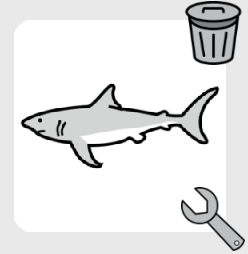
\includegraphics[width=0.3\textwidth]{figures/img/screenshots/sequence_pictogram.png} 
    \caption{A screenshot of a sequence thumbnail as viewed by a guardian.}
    \label{fig:seq_wrench} 
    \vspace{10pt}
\end{wrapfigure}
\bigskip
\noindent
In order to solve this problem firstly we go through the code looking for the implementation of both the bin and the wrench realising that these are both implemented as buttons.
These buttons will henceforth be referred to as the delete and the edit button respectively.
The method \texttt{setupAdapter(final Sequence seq)}, which creates the button view, also calls and overrides the methods that provide their functionality, however no such method is called for the edit button.
An inspection of the code reveals that not only is no such method called, but no such method exists despite the following comment to the method ``\/\/Adds a Delete \& Edit Icon to all Frames which deletes or edits the relevant Frame on click.''.

With the point of failure located a number of solutions present themselves, the fast solution would be to simply write the code as part of the \texttt{setupAdapter} method however this would not be in line with the structure that exists within the sequence code.
Another solution is to find the functionality for when the thumbnail is tabbed and simply copy that, which would be more in line with the structure of the code, yet not be the proper solution.
In order to provide a proper solution which would provide the correct functionality while also maintaining how the rest of sequence has been implemented one could reverse engineer the delete button and use that to construct the proper structure for implementing the edit button.
In order to keep the code maintainable the third option is the solution that we will use, despite knowing it will take more time than the others to implement.

Through further inspection of the code it shows that buttons in sequence are implemented using listeners.
They consist of a handler used to specify the type of click, \texttt{setupOnEditClickHandler()}, an interface with the method \texttt{onEditClick()} and lastly a method, \texttt{setOnEditClickListener(OnEditClickListener listener)}, used to set functionality for the button by overriding \texttt{onEditClick()} when used in order to specify what the button should do at any particular instance.

By creating those three methods and subsequently calling and overriding \texttt{onEditClick()} in the previously mentioned method \texttt{setupAdapter(final Sequence seq)} the issue is fixed without creating any complications.
4 EP is spend on solving the task, mostly on overriding \texttt{onEditClick()} as finding the correct code segments is a lengthy process for while they exist, they were not used until this fix.
